\documentclass[11pt,a4paper]{article}

\usepackage[margin=1in]{geometry}
\usepackage{amsmath,amssymb}
\usepackage{booktabs}
\usepackage{array}
\usepackage{tabularx}
\usepackage{longtable}
\usepackage{graphicx}
\usepackage{float}
\usepackage{xcolor}
\usepackage{hyperref}
\usepackage{enumitem}
\usepackage{listings}
\usepackage{url}

\hypersetup{
    colorlinks=true,
    linkcolor=blue,
    urlcolor=blue,
    citecolor=blue
}

\lstset{
    basicstyle=\ttfamily\small,
    breaklines=true,
    frame=single,
    columns=fullflexible
}

\newcommand{\placeholderfigure}[2]{
\begin{figure}[H]
    \centering
    \fbox{
        \begin{minipage}[c][0.24\textheight][c]{0.88\linewidth}
            \centering
            \textbf{Figure Placeholder}\\[0.5em]
            #2
        \end{minipage}
    }
    \caption{#1}
\end{figure}
}

\title{\textbf{StudyAssistant: A Retrieval-Augmented NLP System for Learning from Lecture PDFs}}
\author{
    Natural Language Processing Project Report\\
    \textit{Student: [Your Name]}\\
    \textit{Instructor: [Instructor Name]}
}
\date{\today}

\begin{document}

\maketitle

\begin{abstract}

StudyAssistant is a retrieval-augmented natural language processing system
designed to support students in learning from lecture PDF documents. The system
takes a collection of course materials as input, extracts and preprocesses their
textual content, builds searchable representations, retrieves relevant evidence
for a user query, and generates grounded learning outputs such as answers,
summaries, quizzes, and flashcards.

Instead of using a large language model as a standalone answer generator, the
project treats generation as the final stage of a broader NLP pipeline. The
pipeline includes PDF text extraction, structure-preserving cleaning, semantic
chunking, lexical retrieval, dense retrieval, hybrid retrieval fusion,
cross-encoder reranking, source-marked prompt construction, and citation
validation. This design aims to make the generated outputs more traceable to
the original lecture materials and reduce unsupported responses.
The project also includes an experimental and ablation framework to analyze the
effect of different retrieval and ranking components on system performance.
The evaluation focuses on whether the system can retrieve relevant evidence,
produce useful learning-oriented outputs, and maintain verifiable source
citations. Overall, StudyAssistant demonstrates how classical information
retrieval, neural retrieval, and grounded language generation can be combined to
build a practical educational assistant for PDF-based course materials.
\end{abstract}

\tableofcontents
\newpage

\section{Introduction}

Lecture materials are increasingly distributed as PDF slide decks, course notes,
and long-form technical documents. Although these materials contain the
knowledge students need, they are not always easy to use during self-study.
Students often need to locate definitions, compare related concepts, understand
formulas, generate summaries before an exam, or create practice questions from
specific topics. Conventional keyword search can help locate pages that contain
matching words, but it does not synthesize information or explain how retrieved
evidence answers a question. General-purpose large language models can produce
fluent explanations, but they may answer from their parametric knowledge rather
than from the course documents. This creates a reliability problem in education:
an answer may sound plausible even when it is unsupported by the uploaded
lecture material.

StudyAssistant addresses this problem using retrieval-augmented generation
(RAG). In a RAG system, the model does not generate an answer directly from its
parameters alone. Instead, the system first retrieves relevant evidence from an
external corpus and then conditions generation on that evidence. This design is
particularly suitable for learning systems because students need answers that
are not only fluent, but also traceable. A useful study assistant should show
which source page supports each answer so that students can inspect the original
lecture slide and verify the explanation. 

The project therefore combines classical information retrieval with neural
retrieval and grounded generation. BM25 is used to capture exact lexical matches
between user questions and lecture terminology. Dense retrieval is used to
capture semantic similarity between paraphrased queries and document chunks.
Hybrid fusion combines both signals, and a cross-encoder reranker improves the
ranking of candidate chunks by jointly scoring query--chunk pairs. Gemini is
used as the generation backend, but the generated output is constrained by a
source-marked context and checked by a citation validation module.

\subsection{Problem Statement}

Let $D = \{d_1, d_2, \ldots, d_n\}$ be a collection of lecture PDF documents.
Each document is processed into a set of chunks
$C = \{c_1, c_2, \ldots, c_m\}$, where each chunk stores text and metadata such
as filename, page number, document id, and chunk id. Given a user query $q$, the
system must retrieve a small ranked set of evidence chunks
$R_q = (c_{r_1}, c_{r_2}, \ldots, c_{r_k})$ and generate an answer $a$ using
only this retrieved evidence.

The answer should satisfy four requirements. \textbf{(i)} It should be relevant to the
query. \textbf{(ii)} It should be faithful to the retrieved context rather than to
unverified model knowledge. \textbf{(iii)} It should contain source markers such as
\texttt{[S1]} and \texttt{[S2]} so that the evidence can be inspected. \textbf{(iv)} If the required information is not present in the retrieved context, the system
should state that the documents do not provide enough information. These
requirements make the task more demanding than ordinary open-ended generation:
the system must perform retrieval, ranking, grounded generation, and citation
validation as a single end-to-end workflow.

\subsection{Contribution}

This project makes the following contributions.

\begin{itemize}
\item It implements a complete PDF-based RAG pipeline for educational
documents, covering document extraction, structure-preserving
preprocessing, semantic chunking, retrieval, reranking, and grounded
generation.

\item It combines lexical and dense retrieval through hybrid score fusion
and further improves context selection using a cross-encoder reranker.

\item It supports multiple learning-oriented tasks, including question
answering, summarization, quiz generation, and flashcard generation, with
source citations for verification.

\item It introduces citation parsing and validation to detect missing or
unsupported citations in generated outputs.

\item It provides a reproducible experimental framework for evaluating
retrieval quality, generation quality, citation correctness, learning
outputs, and ablation settings.

\end{itemize}


\subsection{Task Assignment}

\begin{table}[H]
\centering
\label{tab:task-assignment}
\begin{tabularx}{\textwidth}{p{0.23\linewidth}X p{0.28\linewidth}}
\toprule
Member & Student ID & Tasks \\
\midrule
Pham Thi Ngoc Anh & 20235473 & something \\
Tran Mai Duong & 20235493 & -- \\
Vu Thuy Linh & 20235521 & -- \\
\bottomrule
\end{tabularx}
\end{table}

\subsection{System Overview}

At a high level, the system has two phases. In the offline or indexing phase,
PDF files are extracted page by page and transformed into chunks. Each chunk is
indexed by BM25 and also encoded into a dense vector stored in FAISS. In the
online query phase, a user question is sent to both retrieval systems. BM25
finds chunks with strong lexical overlap, while dense retrieval finds chunks
with high semantic similarity. The two score lists are normalized and fused.
The top candidate chunks are then passed to a cross-encoder reranker, which
selects the final top-$k$ chunks. These chunks are formatted into a prompt with
source markers, and Gemini generates a grounded answer. Finally, the citation
validator checks whether all generated source markers are valid.

\placeholderfigure{High-level StudyAssistant pipeline.}{
Insert a concise left-to-right diagram showing PDF documents, document
processing, dual indexing, hybrid retrieval, reranking, Gemini generation, and
citation validation.
}

\section{Related Work}

This section reviews only the prior work that directly motivates the main
components of the proposed methodology: lexical retrieval, dense retrieval,
retrieval-augmented generation, hybrid retrieval, and reranking.

\subsection{Lexical and Dense Retrieval}

Information retrieval is the first essential component of a document-grounded
question answering system. Classical lexical retrieval methods such as BM25
remain strong baselines because they reward exact term overlap between a query
and a document passage. BM25 improves simple keyword matching by using inverse
document frequency, term-frequency saturation, and document-length
normalization \cite{robertson2009bm25}. This is especially useful for lecture
slides, where important concepts often appear as exact technical terms, such as
`word segmentation'', `dependency parsing'', or ``machine translation''.

However, lexical retrieval alone may fail when the user asks a question using
phrases that do not exactly match the wording in the document. Dense retrieval
addresses this limitation by encoding queries and passages into continuous
vector representations and retrieving passages according to semantic similarity.
Sentence-BERT-style bi-encoders make this efficient by encoding the query and
document chunks separately, allowing fast similarity search over a precomputed
index \cite{reimers2019sentencebert}. In practical systems, vector search
libraries such as FAISS are commonly used to store and search dense embeddings
efficiently \cite{johnson2019faiss}.

\subsection{Retrieval-Augmented Generation}

Retrieval-Augmented Generation (RAG) combines information retrieval with neural
text generation. Instead of asking a language model to answer directly from its
parameters, a RAG system first retrieves relevant passages from an external
document collection and then conditions the generator on those passages
\cite{lewis2020rag}. This design is suitable for educational document systems
because the generated answer should be grounded in the uploaded lecture
materials rather than in unverifiable model knowledge. In this project, RAG is
used as the general framework for question answering, summarization, quiz
generation, and flashcard generation from PDF documents.

\subsection{Hybrid Retrieval and Reranking}

Lexical and dense retrieval capture complementary relevance signals. Lexical
retrieval is effective when the query and document share exact terminology,
while dense retrieval is more flexible for paraphrases and semantic similarity.
Hybrid retrieval combines these signals to improve first-stage candidate
selection. Previous work has also shown that combining retrieval rankings, for
example through Reciprocal Rank Fusion, can outperform individual retrieval
systems \cite{cormack2009rrf}. In this project, hybrid retrieval is implemented
through min-max score fusion between BM25 and dense retrieval scores.

After first-stage retrieval, reranking can further improve the order of
candidate passages. Bi-encoders are efficient but score the query and passage
mostly independently. Cross-encoders instead take the query and passage together
as input, allowing the transformer to model direct token-level interactions
between them. This usually gives more accurate relevance scores, although it is
computationally more expensive \cite{nogueira2019passage}. Therefore, the
proposed pipeline uses cross-encoder reranking only after a limited candidate
set has been retrieved by the hybrid retriever.

\section{Methodology}

\subsection{Document Processing}

\paragraph{PDF Extraction}

StudyAssistant uses \textbf{PyMuPDF} to extract text from PDF files page by page. This is useful because lecture slides are naturally organized by pages, and citations in the system also need to point back to the correct page.

For each PDF file, the system creates a unique document identifier using the SHA1 hash of the file content:

\[
document\_id = \mathrm{SHA1}(\mathrm{file\ bytes})[:16].
\]

This \texttt{document\_id} helps the system recognize and manage each document consistently, even when the pipeline is run multiple times.

After extraction, each page is stored with its \texttt{document\_id}, filename, page number, and extracted text. These metadata are kept throughout the pipeline. Therefore, when a chunk is retrieved later, the system can still know exactly which PDF file and which page it came from. This makes it possible to show citations in the final answer and to evaluate whether retrieval returns the correct source.


\paragraph{Conservative Structure-Preserving Cleaning}

PDF text extraction often produces noisy output, including null characters,
irregular whitespace, broken line endings, and layout artifacts. A very
aggressive cleaning strategy can damage formulas, bullet lists, code fragments,
and table-like slide content. StudyAssistant therefore uses conservative
cleaning. The cleaning stage removes null characters, normalizes line endings,
normalizes repeated spaces inside lines, and preserves paragraph breaks. The
goal is not to reconstruct the visual layout of the PDF, but to preserve enough
textual structure for chunking and generation.

This conservative approach is especially important for lecture slides because
slides often communicate meaning through short lines, bullet hierarchy, and
formula-like text. If preprocessing collapses all line breaks into one long
paragraph, the chunker may combine unrelated items or split meaningful units
incorrectly. By preserving structure, the system gives both retrieval and
generation a better representation of the original learning material.

\paragraph{Semantic Chunking}

Chunking defines the text units that the retrieval system can search and return.
A chunk should contain enough context to be meaningful, but it should not be too
large. If a chunk is too small, it may miss important surrounding information.
If a chunk is too large, it may mix several unrelated concepts and make
retrieval less precise.

StudyAssistant uses \textbf{semantic chunking} instead of cutting text purely by
a fixed number of words. In this approach, the system first splits the extracted
text into smaller semantic units. A semantic unit is a small piece of text that
still carries a relatively complete meaning, such as a paragraph, a sentence, a
bullet point, a line in a slide, or a formula with its explanation. This helps
the system avoid breaking an idea in the middle.

Let a page be represented as a sequence of semantic units:

\[
P = (u_1, u_2, \ldots, u_n).
\]

Here, each $u_i$ is one semantic unit from the page. For example, in a lecture
slide, $u_i$ may correspond to one bullet point or one short explanatory
sentence. Each unit has a word length denoted by $|u_i|.

A chunk $C_j$ is created by grouping several adjacent semantic units together.
The system keeps adding consecutive units until the total length is close to,
but does not exceed, a maximum length budget $L$:

\[
C_j = (u_s, u_{s+1}, \ldots, u_t)
\quad \text{such that} \quad
\sum_{i=s}^{t} |u_i| \leq L.
\]

This means that a chunk is not formed by randomly cutting text at an arbitrary
word position. Instead, it is built from complete semantic units, so the
retrieved chunk is more likely to preserve the original meaning.

To reduce information loss at chunk boundaries, we also uses
overlap. Specifically, the system carries the last $O$ words from the previous
chunk into the next chunk.
This overlap is useful when an important explanation is located near the end of
one chunk and continues in the next one. By sharing a small amount of text
between neighboring chunks, the system reduces the chance that retrieval misses
important context.


\begin{figure}[htbp]
  \centering
  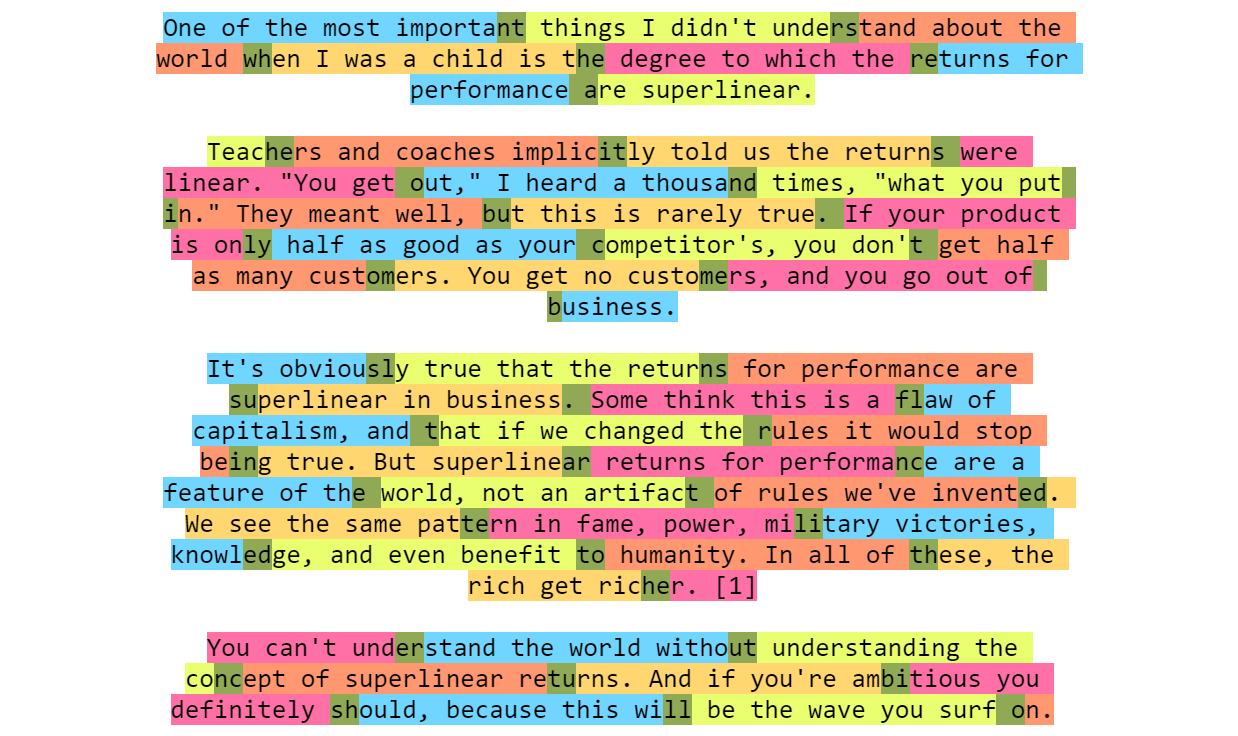
\includegraphics[width=0.85\textwidth]{figures/chunking.png}
  \caption{Chunking with Overlapping.}
\end{figure}


\subsection{Indexing}

\paragraph{BM25 Lexical Index}

The lexical index is built using BM25, a classical ranking function for
keyword-based information retrieval. BM25 estimates how relevant a chunk is to a
query based on exact term overlap between query terms and chunk terms. For a
query $q$ and a chunk $c_i$, BM25 is computed as:

\[
s_{BM25}(q,c_i) =
\sum_{t \in q}
IDF(t)
\frac{f(t,c_i)(k_1 + 1)}
{f(t,c_i) + k_1\left(1 - b + b\frac{|c_i|}{avgdl}\right)}.
\]

Here, $f(t,c_i)$ is the frequency of term $t$ in chunk $c_i$, $|c_i|$
is the length of the chunk, and $avgdl$ is the average chunk length in the
corpus. The parameter $k_1$ controls how much repeated occurrences of a term
increase the score, while $b$ adjusts the effect of chunk length. In other
words, BM25 gives higher scores to chunks that contain important query terms,
but it also prevents very long chunks or repeated words from being unfairly
favored.

The inverse document frequency term is:

\[
IDF(t) =
\log
\frac{N - n_t + 0.5}{n_t + 0.5},
\]

where $N$ is the total number of chunks and $n_t$ is the number of chunks
containing term $t$. This term gives more weight to rare and informative
words, while reducing the impact of common words. BM25 is included because
lecture questions often use the same technical vocabulary as the slides, so
exact term matching remains an important retrieval signal.

\paragraph{Dense Semantic Index}

For semantic retrieval, each chunk is encoded into a dense vector using a SentenceTransformer model. Unlike BM25, which relies on exact keyword overlap, dense retrieval represents the meaning of a query and a chunk in a continuous vector space. This allows the system to retrieve relevant chunks even when the query and the document use different wording.

For each chunk $c_i$ and query $q$, the encoder $E(\cdot)$ produces their vector representations:

\[
\mathbf{c}_i = E(c_i), \qquad \mathbf{q} = E(q).
\]

Before computing similarity, the embeddings are normalized:

\[
\tilde{\mathbf{c}}_i =
\frac{\mathbf{c}_i}{\|\mathbf{c}_i\|_2},
\qquad
\tilde{\mathbf{q}} =
\frac{\mathbf{q}}{\|\mathbf{q}\|_2}.
\]

Normalization ensures that similarity is based mainly on the direction of the vectors rather than their magnitude. The dense retrieval score is then computed by the inner product between the normalized query vector and each normalized chunk vector:

\[
s_{dense}(q,c_i) =
\tilde{\mathbf{q}}^{\top}\tilde{\mathbf{c}}_i.
\]

Because both vectors are normalized, this inner product is equivalent to cosine similarity. A higher score means that the query and the chunk are semantically closer. The chunk vectors are stored in \textbf{FAISS} \texttt{IndexFlatIP}, which performs exact inner-product search. This is suitable for the current corpus size because it gives deterministic retrieval results and avoids approximation errors during evaluation.

\subsection{Retrieval and Fusion}

\paragraph{Candidate Retrieval}

At query time, the system retrieves candidate chunks using both BM25 and dense
retrieval. BM25 produces a lexical score list $s_{BM25}(q,c_i)$, while dense
retrieval produces a semantic score list $s_{dense}(q,c_i)$. These scores are
not directly comparable because they are computed in different ways and usually
have different value ranges. For example, BM25 scores depend on term frequency
and document statistics, while dense scores are based on vector similarity.
Therefore, each score list is min-max normalized:

\[
\hat{s}(q,c_i) =
\frac{s(q,c_i) - \min_j s(q,c_j)}
{\max_j s(q,c_j) - \min_j s(q,c_j) + \epsilon}.
\]

This normalization maps each score list into a comparable range. As a result,
neither BM25 nor dense retrieval dominates the fusion step only because its raw
score values are numerically larger. Instead, the normalized scores reflect the
relative ranking strength of each chunk within the corresponding retrieval
method.

\paragraph{Hybrid Min-Max Score Fusion}

The final first-stage retriever uses hybrid min-max fusion:

\[
    s_{hybrid}(q,c_i) =
    \alpha \hat{s}_{dense}(q,c_i)
    +
    (1-\alpha)\hat{s}_{BM25}(q,c_i).
\]

The parameter $\alpha$ controls the balance between semantic and lexical
retrieval. When $\alpha=0$, the system behaves like normalized BM25. When
$\alpha=1$, the system behaves like normalized dense retrieval. This fusion is useful because lexical and semantic retrieval capture different
types of relevance. BM25 is effective when the query and the document share
exact technical terms, while dense retrieval can find relevant chunks with
similar meaning even when the wording is different. By combining both scores,
the system can produce a more balanced candidate ranking before the reranking
stage.

\paragraph{Cross-Encoder Reranking}

After hybrid retrieval, the system obtains a set of candidate chunks that are
likely to be relevant to the query. However, the first-stage retriever may not
always rank the best chunk at the top. Therefore, StudyAssistant applies a
cross-encoder reranker to refine the ranking of these candidates.

Unlike BM25 or dense retrieval, the cross-encoder reads the query and each
candidate chunk together as a single input. This allows the model to compare
the query and the chunk more carefully and capture detailed interactions between
their words. As a result, it can assign a more accurate relevance score to each
candidate chunk.
The reranker then sorts the candidate chunks according to these relevance
scores and returns the final $top-k$ chunks for generation. This step is more
computationally expensive than first-stage retrieval, because each query--chunk
pair must be scored separately. However, it can improve the quality of the final
context by moving more relevant chunks closer to the top.


\subsection{Grounded Generation}

\subsubsection{Context Construction with Source Markers}

After retrieval and reranking, the system obtains the final top-(k) chunks
that are considered most relevant to the user query. These chunks are then
converted into a source-marked context before being sent to the generation
model. Each chunk is assigned a source marker such as \texttt{[S1]},
\texttt{[S2]}, or \texttt{[S3]}. In addition to the chunk text, the context also
keeps important metadata, including the original filename and page number.

This format serves two purposes. First, it gives the language model a clear and
structured input, where each evidence chunk is separated and identifiable.
Second, it makes the final answer easier to verify, because each cited claim can
be traced back to a specific source marker, PDF file, and page number.

\subsubsection{Gemini Grounded Generation}

We uses Gemini 2.5 Flash as the default generation backend. Instead
of allowing the model to answer freely from its internal knowledge, the system
provides the retrieved source-marked context as the factual basis for
generation. The prompt instructs the model to answer only using the provided
context, cite important claims with source markers, and refuse to answer when
the retrieved context does not contain enough information.

In this setting, generation is treated as a grounded answer construction step.
The model receives the user query and the retrieved context, then produces an
answer that should be both relevant to the query and supported by the given
sources. This design does not completely eliminate hallucination, because a
language model can still misinterpret or overextend the provided context.
However, it reduces unsupported generation by explicitly constraining the model
to the retrieved evidence and by requiring source markers in the output.

\subsection{Citation Validation}

After the answer is generated, we applies a citation validation step
to check whether the model followed the citation protocol. The system extracts
all source markers appearing in the generated answer, such as \texttt{[S1]} or
\texttt{[S2]}, and compares them with the valid source markers that were
actually included in the retrieved context.

This validation focuses on two basic citation requirements. First, the answer
should contain at least one citation when it makes factual claims. This is
called citation coverage. If the model gives an answer without any source
marker, the system marks it as a missing-citation case. Second, every generated
source marker must exist in the retrieved context. This is called citation
validity. If the model cites a marker such as \texttt{[S5]} when only
\texttt{[S1]}, \texttt{[S2]}, and \texttt{[S3]} were provided, the citation is
invalid.

This step is useful because language models may sometimes omit citations or
invent source markers that were not present in the prompt. Citation validation
does not prove that every generated claim is fully correct, since a valid marker
can still be used for an unsupported statement. However, it provides a simple
and deterministic safeguard against marker-level citation errors, improves
transparency, and makes citation failures measurable during evaluation.


\section{Experiments}

\subsection{Experimental Setup}

\subsubsection{Corpus and Benchmark}

\subsection{Evaluation Corpus and Benchmark}

The evaluation uses two corpus settings. Corpus A is the main
lecture-slide corpus, it contains nine NLP
lecture PDFs covering introduction, language modeling, word segmentation,
part-of-speech tagging, dependency parsing, lexical semantics, machine
translation, summarization, and question answering. Corpus A is used for the main
retrieval evaluation, retrieval-component ablation, hybrid alpha ablation,
cross-encoder reranking ablation, citation validation, and error analysis.

Corpus B} is a long-document robustness corpus built from
\texttt{DL\_LectureNotes.pdf}. It is used for the chunking strategy and
chunk-size ablations because a long PDF makes the effect of chunk boundaries more
visible than short lecture-slide pages.

Two benchmark files were created for these corpora: Corpus A contains 120 questions,
including 100 answerable questions with gold source pages and 20 unanswerable
questions. Corpus B contains 35 answerable questions with page-level gold
sources. Both benchmarks follow the same schema: \texttt{question,answer,relevant\_pages,relevant\_chunk\_ids,question\_type}

\subsubsection{Evaluation Metrics}

Retrieval is evaluated using Recall@k, Precision@k, MRR@k, nDCG@k, and latency.
Let $Rel(q)$ be the set of relevant chunks or pages for query $q$, and let
$TopK(q)$ be the ranked set of the top-$k$ retrieved chunks.

Recall@k measures whether relevant evidence is retrieved:

\[
    Recall@k(q) =
    \frac{|TopK(q) \cap Rel(q)|}{|Rel(q)|}.
\]

Because the current benchmark usually has one gold page per question, Recall@k
is numerically equivalent to Hit@k in most cases:

\[
    Hit@k(q) =
    \mathbb{I}(|TopK(q) \cap Rel(q)| > 0).
\]

Recall@k is selected as the primary retrieval metric because RAG generation can
only be grounded if the correct evidence is present in the retrieved context.

Precision@k measures the proportion of retrieved chunks that are relevant:

\[
    Precision@k(q) =
    \frac{|TopK(q) \cap Rel(q)|}{k}.
\]

Precision@k is useful because a RAG prompt with many irrelevant chunks can
distract the generator even if one relevant chunk is present.

MRR@k measures how early the first relevant chunk appears:

\[
    MRR@k =
    \frac{1}{|Q|}
    \sum_{q \in Q}
    \frac{1}{rank_q},
\]

where $rank_q$ is the rank of the first relevant item within the top-$k$ list.
If no relevant item appears, the reciprocal rank is zero. MRR is selected
because the first relevant chunk often has the strongest influence on the final
answer.

nDCG@k is a ranking-sensitive metric that discounts relevant items appearing
lower in the list:

\[
    DCG@k =
    \sum_{i=1}^{k}
    \frac{rel_i}{\log_2(i+1)},
    \qquad
    nDCG@k =
    \frac{DCG@k}{IDCG@k}.
\]

Here $rel_i$ is the relevance value at rank $i$, and $IDCG@k$ is the best
possible discounted gain. nDCG is selected because a RAG system benefits not
only from retrieving evidence, but from placing the best evidence near the top
of the context.

Latency is measured in milliseconds per query. It is included because the
system is intended to support an interactive Streamlit demo, where very slow
retrieval reduces usability.

\subsection{Main Evaluation}

The final retrieval pipeline uses semantic chunking, BM25 and dense retrieval,
hybrid min-max fusion with $\alpha = 0.7$, and cross-encoder reranking over 30
candidate chunks. Table \ref{tab:main-retrieval} reports the aggregate
retrieval performance on 100 benchmark questions.

\begin{table}[H]
\centering
\caption{Final retrieval pipeline performance.}
\label{tab:main-retrieval}
\begin{tabular}{lccccc}
\toprule
Pipeline & Recall@5 & MRR@5 & Precision@5 & nDCG@5 & Latency (ms) \\
\midrule
Hybrid + Reranker & 0.890 & 0.788 & 0.178 & 0.814 & 645.2 \\
\bottomrule
\end{tabular}
\end{table}

The final retriever retrieves a relevant source page within the top five chunks
for 89\% of benchmark questions. The MRR@5 of 0.788 indicates that relevant
evidence is usually ranked near the top after reranking. Precision@5 remains
low because the benchmark normally contains only one gold page per question; if
only one of five retrieved chunks can be counted as relevant, the maximum
single-label precision is 0.2. Therefore, low Precision@5 does not necessarily
mean the remaining chunks are useless; some may be topically relevant but not
listed as gold labels.

\begin{table}[H]
\centering
\caption{Final retrieval performance by question type. The current benchmark
does not yet include question-type labels, so all rows are aggregated under
\texttt{unknown}.}
\label{tab:by-type}
\begin{tabular}{lccccc}
\toprule
Question Type & Num. Questions & Recall@5 & MRR@5 & Precision@5 & nDCG@5 \\
\midrule
Unknown & 100 & 0.890 & 0.788 & 0.178 & 0.814 \\
Comparison  & 3  & 1.000 & 1.000 & 0.200 & 1.000 \\
Definition  & 53 & 0.962 & 0.847 & 0.192 & 0.876 \\
Explanation & 16 & 0.750 & 0.688 & 0.150 & 0.704 \\
Factual     & 28 & 0.821 & 0.713 & 0.164 & 0.740 \\
\bottomrule
\end{tabular}
\end{table}

\subsection{Ablation Study}

\subsubsection{Ablation 1: Chunk Size and Overlap}

This ablation evaluates chunk size and overlap while keeping semantic chunking,
hybrid retrieval, and reranking disabled.
{\small
\begin{table}[H]
\centering
\caption{Chunk size and overlap ablation.}
\label{tab:chunk-size}
\begin{tabular}{ccccccc}
\toprule
Chunk Size & Overlap & Recall@5 & MRR@5 & Precision@5 & nDCG@5 & Latency (ms) \\
\midrule
300  & 50  & 0.457 & 0.314 & 0.091 & 0.350 & 20.4 \\
500  & 80  & 0.657 & 0.380 & 0.131 & 0.448 & 23.2 \\
700  & 100 & 0.657 & 0.396 & 0.131 & 0.461 & 24.4 \\
\bottomrule
\end{tabular}
\end{table}
}

The results show that very small chunks, such as 300 words with 50-word overlap,
perform worse than larger chunk settings. Increasing the chunk size from 300 to
500 improves Recall@5 from 0.457 to 0.657, suggesting that larger chunks provide
more complete context for retrieval. However, after the chunk size reaches 700
words, the retrieval scores become almost unchanged. This indicates that, for
the current corpus, chunk sizes larger than 700 words do not bring additional
retrieval benefits. Therefore, the final system uses 700-word chunks with
100-word overlap as a balanced configuration.


\subsubsection{Ablation 2: Retrieval Component}

This ablation evaluates BM25 only, dense retrieval only, and hybrid min-max
fusion. Reranking is disabled so that the contribution of the first-stage
retriever can be isolated.

\begin{table}[H]
\centering
\caption{Retrieval component ablation.}
\label{tab:retrieval-component}
\begin{tabular}{lccccc}
\toprule
Retrieval Method & Recall@5 & MRR@5 & Precision@5 & nDCG@5 \\
\midrule
BM25 only & 0.700 & 0.581 & 0.140 & 0.611 \\
Dense only & 0.690 & 0.490 & 0.138 & 0.539 \\
Hybrid Min-Max & 0.830 & 0.660 & 0.166 & 0.703 \\
\bottomrule
\end{tabular}
\end{table}

BM25 slightly outperforms dense retrieval on MRR@5 and nDCG@5, showing that
exact terminology is important in this lecture-slide benchmark. However, hybrid
retrieval clearly outperforms both individual retrievers. This supports the
design decision to combine lexical and semantic signals: BM25 captures exact
course terms, while dense retrieval contributes paraphrase and semantic
matching.

\subsubsection{Ablation 4: Hybrid Alpha}

This ablation tunes the hybrid fusion weight $\alpha$. The value $\alpha=0$
corresponds to pure BM25, and $\alpha=1$ corresponds to pure dense retrieval.

\begin{table}[H]
\centering
\caption{Hybrid alpha ablation.}
\label{tab:alpha}
\begin{tabular}{cccccc}
\toprule
$\alpha$ & Recall@5 & MRR@5 & Precision@5 & nDCG@5 & Latency (ms) \\
\midrule
0.0 & 0.700 & 0.581 & 0.140 & 0.611 & 16.4 \\

0.1 & 0.740 & 0.607 & 0.148 & 0.640 & 16.6 \\

0.3 & 0.790 & 0.641 & 0.158 & 0.678 & 16.4 \\

0.5 & 0.790 & 0.641 & 0.158 & 0.679 & 16.4 \\

0.7 & 0.830 & 0.660 & 0.166 & 0.703 & 16.4 \\

0.8 & 0.820 & 0.624 & 0.164 & 0.673 & 16.5 \\

1.0 & 0.690 & 0.490 & 0.138 & 0.539 & 16.8 \\
\bottomrule
\end{tabular}
\end{table}

The results show that combining lexical and dense retrieval is better than using either component alone. When $\alpha=0$, the system relies only on BM25, while when $\alpha=1$, it relies only on dense retrieval. Both settings perform worse than the hybrid configurations. The best Recall@5 and nDCG@5 are obtained at $\alpha=0.7$, while the best MRR@5 is obtained at $\alpha=0.6$. Since $\alpha=0.7$ gives the highest Recall@5 and nDCG@5 with almost the same latency as other settings, it is selected as the final fusion weight.

\subsubsection{Ablation 5: Cross-Encoder Reranking}

This ablation evaluates whether cross-encoder reranking improves the final
ranking. The no-rerank row uses hybrid min-max retrieval with $\alpha=0.7$.
The rerank-30 row uses the final pipeline setting, where the top 30 hybrid
candidates are reranked to produce the final top five. Other candidate sizes are
defined in the experiment script but have not yet been executed.

\begin{table}[H]
\centering
\caption{Cross-encoder reranking ablation.}
\label{tab:reranker}
\begin{tabular}{lcccccc}
\toprule
Setting & Candidate K & Recall@5 & MRR@5 & Precision@5 & nDCG@5 & Latency (ms) \\
\midrule
No rerank & -- & 0.830 & 0.660 & 0.166 & 0.703 & 39.8 \\
Rerank & 10 & 0.840 & 0.759 & 0.168 & 0.779 & 217.3 \\
Rerank & 20 & 0.880 & 0.786 & 0.176 & 0.810 & 345.6 \\
Rerank & 30 & 0.890 & 0.788 & 0.178 & 0.814 & 596.2 \\
Rerank & 50 & 0.880 & 0.785 & 0.176 & 0.809 & 1028.0 \\
\bottomrule
\end{tabular}
\end{table}


Reranking with 30 candidates improves Recall@5 from 0.830 to 0.890 and MRR@5
from 0.660 to 0.788. This means that relevant chunks often appear in the
candidate pool but not necessarily in the first-stage top five. The
cross-encoder can move these relevant chunks upward. The trade-off is latency:
average retrieval time increases from about 23 ms to about 645 ms per query.
This is acceptable for offline experiments and may be acceptable for a demo, but
it should be evaluated carefully for interactive use.

\subsection{Final Configuration for Demo}

Unless a component is being ablated, the default configuration is shown in
Table \ref{tab:final-config}.

\begin{table}[H]
\centering
\caption{Final experiment configuration.}
\label{tab:final-config}
\begin{tabular}{ll}
\toprule
Parameter & Value \\
\midrule
Chunking & Semantic chunking \\
Chunk size & 1000 words \\
Chunk overlap & 150 words \\
Embedding model & \texttt{paraphrase-multilingual-MiniLM-L12-v2} \\
FAISS index & \texttt{IndexFlatIP} with normalized vectors \\
Fusion & Hybrid min-max score fusion \\
Hybrid $\alpha$ & 0.7 \\
Candidate pool & 30 \\
Reranker & \texttt{cross-encoder/ms-marco-MiniLM-L-6-v2} \\
Final top-$k$ & 5 \\
Generator & Gemini 2.5 Flash \\
\bottomrule
\end{tabular}
\end{table}

\subsection{Demo Application}

To demonstrate the final pipeline in an interactive setting, the project includes
a local Streamlit application implemented in \texttt{app.py}. The demo is
designed as a lightweight NotebookLM-style study assistant for lecture PDFs. It
allows a user to upload one or more text-based PDF documents, configure retrieval
settings, ask natural-language questions, inspect retrieved sources, and
generate study materials from the uploaded content.

The demo follows the same retrieval and grounding design as the experimental
pipeline. Uploaded PDFs are processed with PyMuPDF, cleaned, chunked, and indexed
with BM25 and dense vector retrieval. At query time, the user can select the
final retrieval pipeline or inspect individual retrieval modes such as BM25,
dense retrieval, and hybrid retrieval. The final mode applies hybrid min-max
fusion followed by cross-encoder reranking before constructing the source-marked
context for generation.

\begin{table}[H]
\centering
\caption{Main functions exposed in the Streamlit demo.}
\label{tab:demo-functions}
\begin{tabularx}{\linewidth}{p{0.22\linewidth}X}
\toprule
Demo Tab & Functionality \\
\midrule
Q\&A &
Retrieves relevant chunks for a user question and, when a Gemini API key is
provided, generates a cited answer grounded in the retrieved context. \\
Extract &
Extracts requested information such as definitions, formulas, or key facts from
retrieved lecture content. \\
Summarize &
Generates either a query-focused summary or a full-document summary using the
retrieved or selected document chunks. \\
Quiz &
Creates multiple-choice questions with four answer options, a correct answer
index, explanation, and source markers. \\
Flashcards &
Creates front/back study cards with optional hints and source markers for
revision. \\
Debug retrieval &
Shows retrieved chunks and scores for different retrieval methods, making the
retrieval behavior transparent during testing. \\
\bottomrule
\end{tabularx}
\end{table}

The sidebar exposes the main experimental parameters, including chunk size,
chunk overlap, chunking strategy, retrieval method, hybrid alpha, candidate
pool, rerank candidate count, final top-$k$, embedding model, BM25 tokenizer, and
the optional \texttt{GOOGLE\_API\_KEY}. This makes the demo useful not only for
showing the final system, but also for qualitatively inspecting how different
retrieval settings affect the returned evidence.

The local demo can be started from the project root with:

\begin{lstlisting}
.venv/bin/python -m streamlit run app.py
\end{lstlisting}

After startup, the application is available in a browser at
\texttt{http://localhost:8501}. If no Gemini API key is configured, the demo can
still process PDFs and display retrieved sources; generation features are
enabled after the key is provided.

\section{Conclusion}

StudyAssistant demonstrates a complete retrieval-augmented NLP system for
learning from lecture PDF documents. The system combines PDF extraction,
conservative cleaning, semantic chunking, BM25 lexical retrieval, dense
retrieval with SentenceTransformer embeddings, FAISS exact vector search,
hybrid min-max score fusion, cross-encoder reranking, Gemini grounded
generation, and citation validation. The implementation therefore covers both
classical information retrieval and modern neural retrieval/generation
techniques.

The experimental results show that hybrid retrieval is stronger than BM25-only
or dense-only retrieval on the current benchmark. BM25 remains competitive
because lecture slides contain exact technical terms, but dense retrieval adds
useful semantic evidence. The best hybrid setting is around $\alpha=0.6$ to
$0.7$, depending on whether MRR@5 or nDCG@5 is prioritized. Adding cross-encoder
reranking further improves ranking quality, raising Recall@5 to 0.890 and
nDCG@5 to 0.814. The cost is substantially higher latency, so reranking is a
quality--speed trade-off.

The ablation studies also show that chunk size and chunking strategy have
little effect on the current lecture-slide corpus. This is because most slide
pages are short, producing nearly one chunk per page. This result is still
informative because it clarifies that the benchmark is dominated by page-level
slide structure. For longer documents, semantic chunking and chunk size are
expected to matter more.

Overall, the project shows that a responsible educational assistant should not
depend only on a large language model. Retrieval, ranking, prompt construction,
and citation validation are essential components for making answers traceable
to course material.

\section{Limitations}

The current project has several limitations. First, the benchmark contains 100
questions and mostly page-level labels. Page-level relevance is useful for
lecture slides, but it is less precise than chunk-level annotation. A retrieved
chunk may be educationally relevant even when it does not match the exact gold
page, and the current metrics would still count it as incorrect. Future work
should add chunk-level labels and allow multiple gold sources per question.

Second, the current benchmark file does not yet include question-type labels.
As a result, the retrieval-by-type analysis is reported under the generic label
\texttt{unknown}. Adding labels such as definition, factual, explanation,
comparison, multi-hop, and unanswerable would make the evaluation more
diagnostic.

Third, the generation experiments have only been executed as a small one-question
smoke test in the current output directory. Exact Match, Token F1,
answerability accuracy, citation validity, and latency are therefore reported
only as preliminary end-to-end QA indicators. A full generation evaluation should
run the complete benchmark or a larger fixed subset and should manually annotate
groundedness. Without this step, the report can fully evaluate retrieval and
ablation behavior but only partially evaluate end-to-end answer quality.

Fourth, the system uses text extraction only. It does not process figures,
diagrams, screenshots, equations rendered as images, or complex table layouts.
Some lecture slides may contain important information that is not recoverable
from text extraction alone. Future work could add OCR, layout-aware parsing, and
multimodal retrieval.

Fifth, cross-encoder reranking improves retrieval quality but increases latency.
The final deployment should choose between always enabling reranking, enabling
it only for difficult queries, or making it an optional high-accuracy mode.

\section{References}

\begin{thebibliography}{99}

\bibitem{robertson2009bm25}
S. Robertson and H. Zaragoza.
\newblock The Probabilistic Relevance Framework: BM25 and Beyond.
\newblock \textit{Foundations and Trends in Information Retrieval}, 2009.

\bibitem{reimers2019sentencebert}
N. Reimers and I. Gurevych.
\newblock Sentence-BERT: Sentence Embeddings using Siamese BERT-Networks.
\newblock \textit{EMNLP-IJCNLP}, 2019.

\bibitem{karpukhin2020dpr}
V. Karpukhin, B. Oguz, S. Min, P. Lewis, L. Wu, S. Edunov, D. Chen, and W. Yih.
\newblock Dense Passage Retrieval for Open-Domain Question Answering.
\newblock \textit{EMNLP}, 2020.

\bibitem{lewis2020rag}
P. Lewis, E. Perez, A. Piktus, F. Petroni, V. Karpukhin, N. Goyal, H. Kuttler,
M. Lewis, W. Yih, T. Rocktaschel, S. Riedel, and D. Kiela.
\newblock Retrieval-Augmented Generation for Knowledge-Intensive NLP Tasks.
\newblock \textit{NeurIPS}, 2020.

\bibitem{johnson2019faiss}
J. Johnson, M. Douze, and H. Jegou.
\newblock Billion-scale similarity search with GPUs.
\newblock \textit{IEEE Transactions on Big Data}, 2019.

\bibitem{cormack2009rrf}
G. V. Cormack, C. L. A. Clarke, and S. Buettcher.
\newblock Reciprocal Rank Fusion Outperforms Condorcet and Individual Rank
Learning Methods.
\newblock \textit{SIGIR}, 2009.

\bibitem{nogueira2019passage}
R. Nogueira and K. Cho.
\newblock Passage Re-ranking with BERT.
\newblock arXiv:1901.04085, 2019.

\bibitem{jarvelin2002ndcg}
K. Jarvelin and J. Kekalainen.
\newblock Cumulated Gain-based Evaluation of IR Techniques.
\newblock \textit{ACM Transactions on Information Systems}, 2002.

\end{thebibliography}

\appendix

\section{Appendix: Implementation and Reproducibility Details}

This appendix records the main experiment artifacts, benchmark schema, prompt
templates, and commands used to reproduce the final evaluation. The goal is to
make the experimental setup inspectable without interrupting the main report.

\subsection{A. Experiment Artifacts}

\begin{table}[H]
\centering
\caption{Main files used by the final evaluation.}
\label{tab:appendix-artifacts}
\begin{tabularx}{\linewidth}{p{0.30\linewidth}X}
\toprule
Artifact & Description \\
\midrule
\texttt{scripts/run\_experiments.py} &
Unified runner for Corpus A, Corpus B, main evaluation, citation validation,
error analysis, and ablation studies. \\
\texttt{benchmarks/corpusA\_benchmark.csv} &
Lecture-slide benchmark with 120 questions: 100 answerable and 20
unanswerable. Used for main retrieval evaluation and Corpus A ablations. \\
\texttt{benchmarks/corpusB\_benchmark.csv} &
Long-document benchmark for \texttt{DL\_LectureNotes.pdf}. Used for chunking
strategy and chunk-size robustness experiments. \\
\texttt{outputs/final\_evaluation/corpusA/} &
Final retrieval results, retrieval-by-type results, citation validation,
retrieval component ablation, alpha ablation, reranker ablation, and error
analysis. \\
\texttt{outputs/final\_evaluation/corpusB/} &
Chunking strategy and chunk-size ablation results for the long-document corpus. \\
\bottomrule
\end{tabularx}
\end{table}

\subsection{B. Final Configuration}

\begin{table}[H]
\centering
\caption{Default configuration used by the final pipeline.}
\label{tab:appendix-final-config}
\begin{tabular}{ll}
\toprule
Component & Setting \\
\midrule
PDF extraction & PyMuPDF page-level extraction \\
Cleaning & Conservative structure-preserving cleaning \\
Chunking & Semantic chunking \\
Chunk size / overlap & 700 words / 100 words \\
Embedding model & \texttt{paraphrase-multilingual-MiniLM-L12-v2} \\
Dense index & FAISS \texttt{IndexFlatIP} with normalized vectors \\
Fusion & Hybrid min-max score fusion \\
Hybrid alpha & 0.7 \\
Reranker & \texttt{cross-encoder/ms-marco-MiniLM-L-6-v2} \\
Rerank candidate pool & 30 candidates reranked to final top 5 \\
\bottomrule
\end{tabular}
\end{table}

\subsection{C. Benchmark Schema}

Both corpus benchmarks use the same CSV schema:

\begin{lstlisting}[caption={Benchmark CSV format.},label={lst:benchmark-schema}]
question,answer,relevant_pages,relevant_chunk_ids,question_type
\end{lstlisting}

If \texttt{relevant\_chunk\_ids} is empty, page-level relevance is used. A
retrieved chunk is counted as relevant when its \texttt{filename:page} matches a
gold source page in \texttt{relevant\_pages}.

\subsection{D. Prompt Templates}

\subsubsection{Question Answering Prompt}

\begin{lstlisting}[caption={Document-grounded question answering prompt.},label={lst:qa-prompt}]
You are a document-grounded study assistant.
Answer the question using ONLY the provided context.
If the answer is not in the context, say that the document does not provide
enough information.
Cite sources using markers like [S1], [S2].
Return readable Markdown:
- Use bullet points when the answer contains multiple facts, reasons, steps,
  definitions, or examples.
- Otherwise use short paragraphs. Do not return one long paragraph.
- Keep each bullet or paragraph concise and cite key claims with [S1], [S2].
- Answer in the same language as the question.

Question:
{question}

Context:
{context}

Answer:
\end{lstlisting}

\subsubsection{Quiz Generation Prompt}

\begin{lstlisting}[caption={Quiz generation prompt.},label={lst:quiz-prompt}]
Create N multiple-choice questions from ONLY the context.
Return valid JSON only:
{
  "items": [
    {
      "question": "...",
      "options": ["A", "B", "C", "D"],
      "correct_index": 0,
      "explanation": "why the answer is correct, with source marker",
      "source_markers": ["S1"]
    }
  ]
}
Every question must be answerable from the context.
\end{lstlisting}

\subsubsection{Flashcard Generation Prompt}

\begin{lstlisting}[caption={Flashcard generation prompt.},label={lst:flashcard-prompt}]
Create N flashcards from ONLY the context.
Return valid JSON only:
{
  "cards": [
    {
      "front": "...",
      "back": "...",
      "hint": "...",
      "source_markers": ["S1"]
    }
  ]
}
\end{lstlisting}

\subsection{E. Reproducibility Commands}

The final evaluation can be reproduced from the project root using:

\begin{lstlisting}[caption={Run all final evaluations and ablations.},label={lst:run-all}]
.venv/bin/python scripts/run_experiments.py all
\end{lstlisting}

To run only the main lecture-slide corpus:

\begin{lstlisting}[caption={Run Corpus A evaluation.},label={lst:run-corpus-a}]
.venv/bin/python scripts/run_experiments.py corpusA
\end{lstlisting}

To run only the long-document chunking robustness experiments:

\begin{lstlisting}[caption={Run Corpus B evaluation.},label={lst:run-corpus-b}]
.venv/bin/python scripts/run_experiments.py corpusB
\end{lstlisting}

Gemini-dependent generation experiments require a configured API key:

\begin{lstlisting}[caption={Run generation evaluation with Gemini enabled.},label={lst:run-generation}]
export GOOGLE_API_KEY="your_api_key"
.venv/bin/python scripts/run_experiments.py corpusA --run-generation
\end{lstlisting}

\end{document}
